\begin{chapter}{Preliminaries}
Throughout the text, $k$ will denote a field of characteristic zero.
\begin{section}{The path algebra of a quiver}
A \emph{quiver} is a quadruple $Q=(Q_0, Q_1, s,t)$, where $Q_0$ and $Q_1$ are finite sets whose elements are called \emph{vertices} and \emph{arrows} respectively, and $s,t:Q_1\to Q_0$ are functions that associate to each arrow $\alpha\in Q_1$ its \emph{source} $s(\alpha)\in Q_0$ and its \emph{target} 
$t(\alpha)\in Q_0$. We will usually abbreviate the fact that an arrow $\alpha\in Q_1$ has source $a$ and target $b$ using the notation $\alpha:a\to b$. We will also omit mentioning $s$ and $t$ explicitly when they are clear from context.

One can represent a quiver graphically as an oriented graph allowing loops and multiple arrows between the same pair of vertices. The following are some examples of quivers:
\textcolor{red}{ejemplo con loops}
\[
\begin{tikzpicture}[->,node distance=1cm, thick]
\tikzstyle{every node} = [circle, fill=gray!30, minimum size=.5cm]
\node (1) {};
\node (2) [right=of 1] {};
\node (3) [right=of 2] {};
\node (4) [right=of 3] {};
\node (5) [right=of 4] {};
\node (6) [right=of 5] {};
\node (7) [right=of 6] {};
\node (8) [below=of 3] {};
\foreach \from/\to in {2/1, 3/2, 3/4, 3/8, 4/5, 5/6, 6/7}
\draw [->] (\from) -- (\to);
\end{tikzpicture}
\]
Let $Q=(Q_0, Q_1, s, t)$ be a quiver and consider the $k$-vector spaces $R=k^{Q_0}$ and $A=k^{Q_1}$, which we will call the \emph{vertex span} and \emph{arrow span} of $Q$, respectively. The space $R$ is a commutative $k$-algebra with the product given by pointwise multiplication. Thus, we can consider an $R$-bimodule structure on $A$ given as follows: if $r\in Q_0$, $\alpha\in Q_1$ then we define $r\alpha = \delta_{r,t(\alpha)} \alpha$ and analogously $\alpha r = \delta_{r, s(\alpha)}\alpha$, and extend the action linearly. That is, a vertex $r$ acts as the identity on the left (right) of an arrow $\alpha$ if the target (source) of $\alpha$ is $r$, and otherwise acts as zero. The \emph{path algebra} $\kQ$ associated to the quiver $Q$ is the graded tensor algebra
$$\kQ = \bigoplus_{n=0}^\infty A^{\otimes_R n},$$
where we set $A^{\otimes_R 0}=R$. For the sake of simplicity we will usually notate $A^{\otimes_R n}$ as $A^n$ and an elementary tensor $\alpha_n\otimes\dots\otimes \alpha_1$ as $\alpha_n\dots\alpha_1$. Notice that a non-zero element of the form $\alpha_n\dots\alpha_1$ consists of a sequence of \emph{concatenable} arrows $\alpha_i$, that is, arrows such that $s(\alpha_{i+1})=t(\alpha_i)$. We will call such an element a \emph{path of length n}. It is worth observing that the collection of all paths of length $n$ form a basis of $A^n$ as a $k$-vector space. Since $Q_0$ is a basis of $A^0=R$, we will consider elements of $Q_0$ as \emph{paths of length 0}, which we will usually call \emph{trivial} or \emph{stationary} paths. Considering $Q_0$ and $Q_1$ are in bijection with paths of length 0 and 1 respectively, we will denote the set of paths of length $n$ as $Q_n$ and the set of all paths as $Q_*$. We can now define source and target functions $s,t:Q_*\to Q_0$ as follows: if $u=\alpha_n\dots\alpha_0\in Q_n$ with $n>0$, then $s(u)=s(\alpha_0)$ and $t(u)=t(\alpha_n)$. Otherwise, if $u=r\in Q_0$ then $s(u)=t(u)=r$. Thus, one easily checks that if $a,b\in Q_0$, the space spanned by paths with source $a$ and target $b$ is exactly $b\kQ a$.

\textcolor{red}{propiedad universal}

Let us consider some examples:
\begin{exmp} Let $Q$ be the quiver with vertices $\{1,\dots,n\}$ and no arrows:
\[
\begin{tikzpicture}[node distance=1cm, auto, thick]
\tikzstyle{every node} = [circle, fill=gray!30, minimum size=.5cm]
\node (1) {1};
\node (2) [right=of 1] {2};
\node (3) [right=of 2] {3};
\node (4) [right=of 3, fill=white] {...};
\node (5) [right=of 4] {n};
\end{tikzpicture}
\]
The path algebra $\kQ$ is then isomorphic to $k^n = ke_1\oplus\dots\oplus ke_n$, where multiplication is given by $e_i e_j = \delta_{i,j} e_i$ and extended linearly.
\end{exmp}

\begin{exmp}\label{one-loop} Let $Q$ be the quiver with a single vertex $1$ and a single arrow $\alpha:1\to 1$:
\[
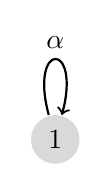
\begin{tikzpicture}[->, thick]
\tikzset{every loop/.style={looseness=15}}
\node[circle, fill=gray!30, minimum size=.5cm]  (1) {1};
\path (1) edge [loop above] node {$\alpha$} (1);
\end{tikzpicture}
\]
The path algebra $\kQ$ has a basis given by $\{e_a, \alpha, \alpha^2, \dots\}$. It is easily seen that $\kQ$ is isomorphic to the polynomial algebra $k[x]$, via the map sending $\alpha \mapsto x$ and $1\mapsto 1$.
\end{exmp}
\begin{exmp}\label{several-loops} More generally, let $Q$ be the quiver with a single vertex $1$ and $n$ arrows $\alpha_n:1\to 1$:
\[
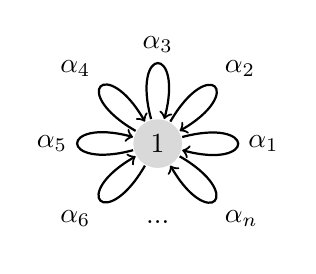
\begin{tikzpicture}[->, auto, thick]
\tikzset{every loop/.style={looseness=15}}
\node[circle, fill=gray!30, minimum size=.5cm]  (1) {1};
\node[circle, fill=white] (2) at +(270: 1) {...};
\path (1) edge [loop left] node {$\alpha_5$} (1);
\path (1) edge [loop above] node {$\alpha_3$} (1);
\path (1) edge [loop right] node {$\alpha_1$} (1);
\path (1) edge [in=30, out=60, loop] node {$\alpha_2$} (1);
\path (1) edge [in=210, out=240, loop] node {$\alpha_6$} (1);
\path (1) edge [in=120, out=150, loop] node {$\alpha_4$} (1);
\path (1) edge [in=300, out=330, loop] node {$\alpha_n$} (1);
\end{tikzpicture}
\]
Then, the path algebra $\kQ$ is isomorphic to the free algebra on $n$ generators $k\langle x_1,\dots, x_n\rangle$, via the map sending $\alpha_i\mapsto x_i$ and $1\mapsto 1$.
\end{exmp}

A path $u\in Q_n$ with $n>1$ such that $s(u)=t(u)$ is called a \emph{cycle}, and a quiver containing no cycles is said to be \emph{acyclic}. As we can infer from the previous examples, the existence of cycles in the quiver is closely related to the dimension of the path algebra. More precisely, we have:

\begin{prop}\label{acyclic-fin-dim}
Let $Q$ be a quiver and $\kQ$ its associated path algebra. Then $\kQ$ is finite-dimensional iff $Q$ is acyclic.
\end{prop}
\begin{proof} Suppose $\kQ$ is infinite-dimensional. Then the set of all paths $Q_*$, which is a basis for $\kQ$, must be infinite. Since the quiver has only a finite number of arrows, there's only a finite number of paths of less than a fixed length. Therefore, if the set of paths $Q_*$ is infinite, then there exist arbitrarily long paths. Let $n$ be the number of vertices in $Q_0$ and pick a path $\alpha_m\dots\alpha_1$ with $m>n$. Then $s(\alpha_i) = t(\alpha_j)$ for some $1\leq i < j\leq m$ and so $\alpha_j\dots\alpha_i$ is a cycle in $Q$.

Conversely, if $Q$ contains a cycle $u$, then $\{u,u^2,u^3,\dots\}$ is an infinite linearly independent set, and so $\kQ$ is infinite-dimensional.
\end{proof}

We now define the \emph{complete path algebra} $\KQ$ associated to a quiver $Q$ as
$$\KQ = \prod_{n=0}^\infty A^n,$$
that is, elements of $\KQ$ are possibly infinitely supported linear combinations of paths in $Q_*$ and the product on $\KQ$ is just the natural extension of the product on $\kQ$.

\textcolor{red}{todo este párrafo debería explicarse mejor una vez que esté hecha la parte del lema topológico} The path algebra $\kQ$ admits a $k$-algebra ultranorm $\vert \cdot \vert: \kQ\to [0, \infty)$ such that for each non-zero $x=\sum_{u\in Q_*} \lambda_u u$ we have $\vert x\vert = e^{-\nu(x)}$, where $\nu(x) = \min\{ i\in \NN_0 : |u| = i \text{ and } \lambda_u \neq 0 \}$. We call this the \emph{$\mathfrak{m}$-adic ultranorm} on $\kQ$. One can check that the complete path algebra $\KQ$ is in fact the completion of the path algebra $\kQ$ with respect to the $\mathfrak{m}$-adic ultranorm.

\begin{exmp}Let $Q$ be an acyclic quiver. As we proved in \ref{acyclic-fin-dim}\textcolor{red}{$\leftarrow$ formatear bien esto}, the associated path algebra $\kQ$ is finite-dimensional, and so $A^n=0$ for big enough $n$. Therefore, $\bigoplus A^n=\prod A^n$ and so the path algebra coincides with its completion.
\end{exmp}

\begin{exmp}Let $Q$ be the quiver from \ref{several-loops}. The isomorphism $\kQ\simeq k\langle x_1,\dots,x_n\rangle$ extends to an isomorphism between the completions $\KQ\simeq k\langle\langle x_1,\dots,x_n\rangle\rangle$, where the right-hand side term is the algebra of non-commutative formal power series in $n$ variables.
\end{exmp}
\end{section}

\begin{section}{The Jacobian algebra of a quiver with potential}
\textcolor{red}{motivación}

Let $Q$ be a quiver and $\KQ=\prod A^n$ its complete path algebra. For $n\geq 1$, we define the \emph{cyclic part} of $A^n$ as
$$A^n_{\cyc} = \bigoplus_{r\in Q_0} rA^nr,$$
that is, the $R$-submodule spanned by cycles of length $n$. A \emph{potential} $S$ is an element of the closed \textcolor{red}{probarlo} $R$-submodule $\KQ_{\cyc}\subseteq \KQ$, which we define as
$$\KQ_{\cyc}=\prod_{n=1}^\infty A^n_{\cyc}$$
In other words, a potential is a possibly infinitely supported linear combination of cycles. We will call a pair $(Q,S)$ a \emph{quiver with potential}, or \emph{QP} for short.

In their work \cite{rota80}, Rota, Sagan and Stein introduced a notion of derivative for non-commutative algebras, called the \emph{cyclic derivative}. Here we will work with this concept within the context of the complete path algebra of a quiver. Given an arrow $\alpha\in Q_1$, the cyclic derivative with respect to $\alpha$ is the morphism $\partial_\alpha:\KQ_\cyc\to \KQ$ defined for a cycle $u=\alpha_n\dots\alpha_1$ as
$$\partial_\alpha(u) = \sum_{k=1}^n \delta_{\alpha, \alpha_k}\alpha_{k+1}\dots\alpha_n\alpha_1\dots\alpha_{k-1}$$
and extended linearly and continuously.

We are now able to introduce the \emph{Jacobian algebra} associated to a QP, which is the main object of study in this thesis. Given a QP $(Q,S)$, the \emph{Jacobian ideal} $J(S)$ is the closed ideal in $\KQ$ generated by the set of all cyclic derivatives of the potential, that is, $\{\delta_\alpha(S) : \alpha\in Q_1\}$. The Jacobian algebra $P(Q,S)$ is then the quotient $\KQ/J(S)$.

\begin{exmp} Let $Q$ be the quiver from \ref{one-loop}. As we have seen, the complete path algebra $\KQ$ is isomorphic to the algebra of formal power series $k\llbracket x\rrbracket$. Identifying $x$ with the only arrow in the quiver, we see that any potential for Q is of the form $\sum_{n=1}^\infty \lambda_n x^n$ for some choice of scalars $\lambda_n\in k$. For example, let us consider the potential $S=x^n$. Since $x$ is the only arrow in the quiver, we just have to compute $\partial_x(x^n)$, which turns out to be $nx^{n-1}$ (happily coinciding with the usual, commutative notion of derivation). Therefore, the Jacobian algebra is $k\llbracket x\rrbracket/(nx^{n-1})$, which is isomorphic to the truncated polynomial algebra $k[x]/(x^{n-1})$.
\end{exmp}

Two potentials $S$ and $S'$ are said to be \emph{cyclically equivalent} if their difference $S-S'$ lies in the closed $k$-subspace spanned by elements of the form $\alpha_n\dots\alpha_1 - \alpha_1\alpha_n\dots\alpha_2$, where $\alpha_n\dots\alpha_1$ is a cycle, or equivalently, if every term of $S$ is a cyclic permutation of the factors of a term of $S'$. \textcolor{red}{habría que definir term y factor o es claro?}. It is easily checked that if $S$ and $S'$ are cyclically equivalent, then $\partial_\alpha(S)$ is just a reordering of the summands of $\partial_\alpha(S')$, and so they coincide. This in turn implies that $S$ and $S'$ induce both the same Jacobian ideal and the same Jacobian algebra.

\begin{exmp} Let $Q$ be the quiver with vertices 1 and 2, and arrows $\alpha:1\to 2$, $\beta:2\to1$:
\[
\begin{tikzpicture}[->,node distance=1cm, thick]
\tikzstyle{every node} = [circle, fill=gray!30, minimum size=.5cm]
\node (1) {1};
\node (2) [right=of 1] {2};
\foreach \from/\to in {2/1, 1/2}
\draw (1.20) -- (2.160) node[midway, above, fill=white] {$\alpha$};
\draw (2.200) -- (1.340) node[midway, below, fill=white] {$\beta$};
\end{tikzpicture}
\]
Any potential for $Q$ is of the form $\sum_{n=1}^\infty \lambda_n (\alpha\beta)^n + \mu_n (\beta\alpha)^n$ for some scalars $\lambda_n, \mu_n\in k$. For instance, the cyclically equivalent potentials $S=(\alpha\beta)^n$ and $S'=(\beta\alpha)^n$ give rise to the same Jacobian ideal, which is $(\partial_\alpha(S), \partial_\beta(S)) = (n(\beta\alpha)^{n-1}\beta, n(\alpha\beta)^{n-1}\alpha)$. As any path of length at least $n$ has either $(\beta\alpha)^{n-1}\beta$ or $(\alpha\beta)^{n-1}\alpha$ as factors, the Jacobian ideal contains $A^d$ for $d\geq n$. Therefore, the Jacobian algebra $P(Q,S)$ turns out to be finite-dimensional.
\end{exmp}

In the context of Jacobian algebras, having finite dimension is a highly desirable attribute. A usual method for showing this, as seen in the works of \textcolor{red}{citas}, consists in showing that enough cycles are contained in the Jacobian ideal, just as we did in the toy example above. We will make use of the diamond lemma in order to produce this kind of arguments in a streamlined fashion.
\end{section}
\end{chapter}